\documentclass[10pt,twocolumn]{article}

% ---------------------------------------------------------------------------
% Packages
% ---------------------------------------------------------------------------
\usepackage[utf8]{inputenc}
\usepackage[T1]{fontenc}
\usepackage{lmodern}
\usepackage[margin=1.9cm,columnsep=0.6cm]{geometry}
\usepackage{graphicx}
\usepackage{booktabs}
\usepackage{caption}
\usepackage{subcaption}
\usepackage{amsmath}
\usepackage{amssymb}
\usepackage{xcolor}
\usepackage{enumitem}
\usepackage{microtype}
\usepackage{float}
\usepackage{titlesec}
\usepackage[hidelinks,colorlinks=true,linkcolor=blue!50!black,citecolor=blue!50!black,urlcolor=blue!50!black]{hyperref}

\graphicspath{{../img/}{../reports/attention/}}

\titlespacing*{\section}{0pt}{2.2ex plus 1ex minus .2ex}{1.3ex plus .2ex}
\titlespacing*{\subsection}{0pt}{1.8ex plus 1ex minus .2ex}{1ex plus .2ex}

\newcommand{\code}[1]{\texttt{\small #1}}

\setlength{\abovecaptionskip}{4pt}
\setlength{\belowcaptionskip}{2pt}
\captionsetup{font=small,labelfont=bf}

% ---------------------------------------------------------------------------
\title{\vspace{-0.5cm}\textbf{SwinAD2Net: A Swin Transformer / Atrous Dense Network Hybrid for Cervical Cytology Classification}\\[2pt]
\large An honest empirical comparison against a DenseNet121-based baseline}
\author{
Richard Viana \\
\small \texttt{cervical\_cancer} project --- \url{https://github.com/rick0110/cervical_cancer}
}
\date{}

\begin{document}
\twocolumn[
  \begin{@twocolumnfalse}
    \maketitle
    \begin{abstract}
    \noindent
    Automated cervical cytology classification can reduce the workload and inter-observer variability of manual Pap-smear screening. This report presents \textbf{SwinAD2Net}, a hybrid architecture that combines Swin Transformer window attention with Atrous Dense Blocks (ADB) and Squeeze-and-Excitation (SE) channel recalibration, and compares it head-to-head with a from-scratch reproduction of \textbf{A2SDNet121}, the DenseNet121-based model proposed by Zhang \emph{et al.}~\cite{zhang2025}. Both models are trained under an identical, compute-constrained protocol (bf16 mixed precision, 3-fold stratified cross-validation, early stopping) on the Herlev and SIPaKMeD datasets, individually and pooled into a shared binary (normal/abnormal) task. A small sequential hyperparameter search selects the best SwinAD2Net configuration before the final comparison. Under this harmonized budget, SwinAD2Net outperforms the A2SDNet121 reproduction on every metric, in every dataset/task combination, while using roughly \textbf{3$\times$ fewer parameters} (2.22M vs.\ 6.87M) --- for example 98.74\% vs.\ 88.94\% accuracy on SIPaKMeD binary classification, and 95.78\% vs.\ 76.19\% on the SIPaKMeD 5-class task. We report this result together with an important caveat: our A2SDNet121 reproduction falls well short of the numbers Zhang \emph{et al.} report for the same architecture (e.g.\ 32.8\% vs.\ their 99.14\% on Herlev 7-class), most plausibly because the original protocol trains for 300 epochs with a schedule tuned specifically for that network, while our budget uses early stopping across ten separate runs. We use Grad-CAM~\cite{selvaraju2017} --- the same diagnostic tool used in the original paper --- to compare where each network attends when making a prediction, finding that A2SDNet121 tends to produce more spatially concentrated saliency maps centered on the nucleus, while SwinAD2Net's attention is measurably more diffuse. However, a genuine self-attention rollout~\cite{abnar2020} computed from SwinAD2Net's own attention weights (impossible for A2SDNet121, which has no self-attention) is consistently \emph{more} concentrated than SwinAD2Net's own Grad-CAM map, and on one dataset is even the most concentrated map of the three --- suggesting that part of the ``diffuse SwinAD2Net'' impression from Grad-CAM alone is an artifact of applying a CNN-native diagnostic to a transformer, not a genuine property of what the network attends to.
    \end{abstract}
    \vspace{0.4cm}
  \end{@twocolumnfalse}
]

% =============================================================================
\section{Introduction}
% =============================================================================

Cervical cancer screening via Pap-smear cytology is one of the most effective cancer-prevention tools in women's healthcare, but manual inspection is labor-intensive, requires specialized training, and is subject to inter- and intra-observer variability. Deep-learning classifiers can act as a triage or second-reader system, flagging likely-abnormal cells for prioritized review and potentially reducing false negatives.

Zhang \emph{et al.}~\cite{zhang2025} recently proposed \textbf{A2SDNet121}, a DenseNet121 backbone augmented with Squeeze-and-Excitation (SE) blocks and Atrous Dense Blocks (ADB) for multi-scale feature extraction, reporting accuracies above 99\% on both the Herlev and SIPaKMeD datasets. DenseNet-style networks are, however, purely convolutional: every layer only ever sees a fixed, local receptive field per operation, and global context has to be built up gradually through depth. Vision Transformers, and in particular the \textbf{Swin Transformer}~\cite{liu2021swin}, instead compute self-attention across explicit spatial windows, giving each layer a much larger effective receptive field per operation, at the cost of transformers' typically larger parameter counts and data requirements.

This project asks a concrete, falsifiable question: \emph{does replacing/augmenting DenseNet-style local feature extraction with Swin window attention improve cervical-cytology classification, under a training budget realistic for a single consumer/workstation GPU, and where does each model actually look when it decides?} We answer this by:

\begin{enumerate}[leftmargin=*,itemsep=1pt,topsep=2pt]
    \item Building \textbf{SwinAD2Net}, a hybrid stage design of Swin blocks $\rightarrow$ ADB $\rightarrow$ SE $\rightarrow$ Transition, in three concrete variants (Section~\ref{sec:variants}), and reproducing \textbf{A2SDNet121} from the paper's description as a baseline (Section~\ref{sec:a2sdnet});
    \item Running a small, strictly \emph{sequential} hyperparameter search (Section~\ref{sec:hpsearch}) to select a competitive SwinAD2Net configuration without hand-tuning;
    \item Training both architectures under one \emph{harmonized} protocol --- same optimizer family knobs, same early-stopping policy, same 3-fold cross-validation --- on Herlev, SIPaKMeD, and a pooled binary task (Section~\ref{sec:protocol});
    \item Reporting results honestly, including where our A2SDNet121 reproduction \emph{fails} to reach the original paper's numbers, and explaining why (Section~\ref{sec:results});
    \item Comparing the two networks' Grad-CAM saliency maps~\cite{selvaraju2017}, plus a genuine self-attention rollout~\cite{abnar2020} native to SwinAD2Net's own mechanism, to see whether they attend to the same cytological structures (Section~\ref{sec:interpretability}).
\end{enumerate}

% =============================================================================
\section{Related Work}
% =============================================================================

\textbf{DenseNet and A2SDNet121.} DenseNet~\cite{huang2016densenet} connects every layer within a block to every subsequent layer via channel-wise concatenation, encouraging feature reuse and mitigating vanishing gradients. Zhang \emph{et al.}~\cite{zhang2025} build on DenseNet121 by inserting an SE block after each dense block (for channel-wise recalibration) and replacing the standard dense blocks with \emph{Atrous} Dense Blocks, where the last few layers of each block use dilated convolutions (rates 1, 2, 3) to widen the receptive field without added downsampling. They report accuracies of 99.75\%/99.14\% for Herlev binary/7-class and 99.55\%/99.75\%/99.22\% for SIPaKMeD binary/3-class/5-class, trained for 300 epochs with SGD (initial LR $10^{-4}$, \code{StepLR} decay) and batch size 8 on an NVIDIA RTX5000.

\textbf{Swin Transformer.} Liu \emph{et al.}~\cite{liu2021swin} restrict self-attention to non-overlapping local windows and alternate a shifted-window partitioning between consecutive blocks so that information still propagates across window boundaries, giving linear (rather than quadratic) complexity in the number of tokens while retaining most of the modeling benefit of full self-attention. This project's window-attention implementation follows the Swin~V2-style refinements of cosine attention with a learned temperature $\tau$ and a log-spaced continuous relative-position bias (a small MLP over relative coordinates), which improve training stability at the window sizes used here.

\textbf{Grad-CAM.} Gradient-weighted Class Activation Mapping~\cite{selvaraju2017} produces a coarse localization heatmap for a target class by weighting the last convolutional (or, here, last spatial pre-pooling) feature map by the class-specific gradients flowing into it. Zhang \emph{et al.} already use Grad-CAM to argue that their SE-augmented model attends more to nuclei than a plain DenseNet121; Section~\ref{sec:interpretability} repeats this diagnostic to compare A2SDNet121 against SwinAD2Net. Because Grad-CAM was designed for CNN feature maps, we complement it with \textbf{attention rollout}~\cite{abnar2020}, which composes a transformer's \emph{own} layer-wise self-attention matrices (with an added residual identity, as in the original formulation) to trace how strongly each output token's representation actually depends on each input token --- a diagnostic with no equivalent for a network, like A2SDNet121, that has no self-attention.

% =============================================================================
\section{Datasets and Tasks}
% =============================================================================

Two public single-cell cervical cytology datasets are used, matching the counts reported by Zhang \emph{et al.}:

\begin{itemize}[leftmargin=*,itemsep=1pt,topsep=2pt]
    \item \textbf{Herlev / MDE-Lab Pap Smear Collection} --- 917 images, 7 fine-grained classes (Normal superficial, Normal intermediate, Normal columnar, Light dysplastic, Moderate dysplastic, Severe dysplastic, Carcinoma in situ); the first three are grouped as \emph{normal}, the rest as \emph{abnormal}.
    \item \textbf{SIPaKMeD} --- 4{,}049 single-cell \code{CROPPED} images, 5 classes (Superficial-Intermediate, Parabasal, Koilocytotic, Dyskeratotic, Metaplastic); Superficial-Intermediate/Parabasal are \emph{normal}, Koilocytotic/Dyskeratotic are \emph{abnormal}, and Metaplastic is benign but conventionally grouped with \emph{abnormal}.
\end{itemize}

Because the two datasets do not share a class taxonomy, two task families are evaluated: a \textbf{binary} normal-vs-abnormal task (evaluable per dataset \emph{and} on a pooled Herlev+SIPaKMeD set of 4{,}966 images, using the shared binary label), and a \textbf{multi-class} task evaluated separately per dataset (7-way for Herlev, 5-way for SIPaKMeD).

\textbf{Why on-the-fly augmentation.} Rather than pre-generating and storing several augmented copies of every training image on disk (a common but I/O- and storage-heavy pattern), augmentation here is applied stochastically \emph{every epoch} via \code{torchvision.transforms} (random-resized crop, horizontal/vertical flip, color jitter, rotation). This gives at least as much effective augmentation diversity across a full training run --- since the network sees a fresh random transform each epoch rather than a fixed finite set of pre-baked variants --- without inflating dataset size, disk usage, or per-epoch I/O.

% =============================================================================
\section{Method: SwinAD2Net Architecture}
% =============================================================================

\begin{figure*}[t]
    \centering
    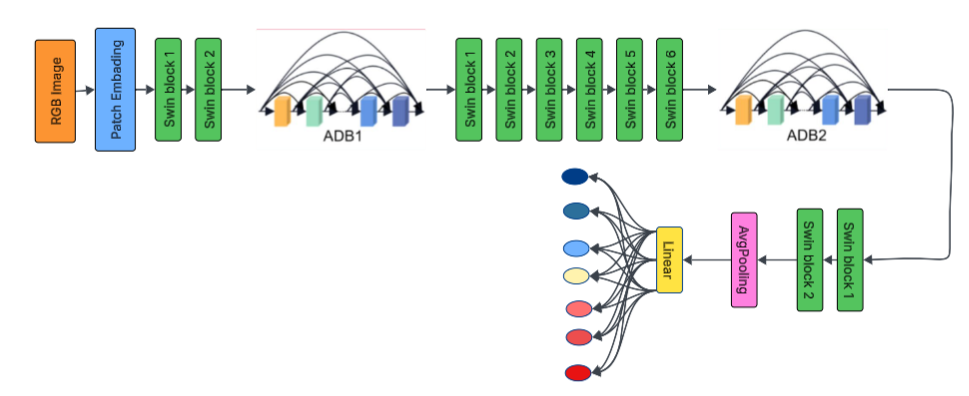
\includegraphics[width=0.92\textwidth]{main_scheme_AD2Net.png}
    \caption{SwinAD2Net stage layout: patch embedding, followed by four repetitions of [Swin Transformer blocks $\rightarrow$ Atrous Dense Block $\rightarrow$ Squeeze-and-Excitation $\rightarrow$ Transition layer] with decreasing spatial resolution, ending in global average pooling and a linear classifier.}
    \label{fig:mainscheme}
\end{figure*}

SwinAD2Net (Figure~\ref{fig:mainscheme}) is built around one repeating stage design applied four times at decreasing spatial resolution ($56{\times}56 \to 28{\times}28 \to 14{\times}14 \to 7{\times}7$ for a 224-pixel input with patch size 4): \textbf{Swin Transformer blocks} for global context, an \textbf{Atrous Dense Block} for multi-scale local feature extraction, a \textbf{Squeeze-and-Excitation} block for channel recalibration, and a \textbf{Transition layer} for downsampling/compression. The design goal is to keep DenseNet's strong local feature reuse while adding a genuine global receptive field per stage, something a purely convolutional stack can only approximate by stacking many layers.

\subsection{Patch Embedding}
A \code{patch\_size}$\times$\code{patch\_size} strided convolution (patch size 4) projects the $224{\times}224{\times}3$ input into non-overlapping \code{embed\_dim}-dimensional patch embeddings, followed by LayerNorm. \textbf{Why a conv instead of a linear patch-flatten-and-project (as in ViT)}: the convolutional formulation is mathematically identical when patches don't overlap, but keeps the implementation naturally compatible with the 4D \code{[B,C,H,W]} tensor layout used by the ADB/SE stages that follow, avoiding constant reshaping between "transformer-token" and "CNN-feature-map" representations throughout the network.

\subsection{Swin Transformer Stage}
\begin{figure}[H]
    \centering
    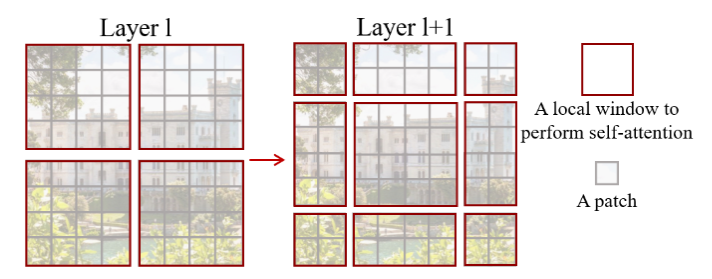
\includegraphics[width=0.95\linewidth]{shift_window.png}
    \caption{Shifted-window partitioning: alternating un-shifted and shifted window layouts let information cross window boundaries across consecutive blocks without full quadratic attention.}
    \label{fig:shiftwindow}
\end{figure}

Each stage contains a pair (or, in stage 3, three pairs) of Swin blocks: one with the standard window partition, one with the windows shifted by half a window size (Figure~\ref{fig:shiftwindow}), so that two consecutive blocks together let every token interact with a neighborhood larger than one window. Within each window, attention uses \textbf{cosine similarity} between $\ell_2$-normalized queries/keys, divided by a learned per-head temperature $\tau$ (clamped $\geq 0.01$), rather than the original dot-product/$\sqrt{d}$ scaling. \textbf{Why cosine attention}: dot-product attention magnitudes can grow unboundedly with training and destabilize optimization at the window sizes and depths used here; bounding the similarity to $[-1/\tau, 1/\tau]$ keeps attention logits well-scaled throughout training. Relative positional information is injected as an additive bias computed by a small 2-layer MLP (\emph{meta-network}) over log-spaced relative coordinates, rather than a fixed lookup table --- \textbf{why}: a continuous MLP bias generalizes to window-size changes and needs far fewer parameters than one learned bias entry per relative-position pair.

\subsection{Atrous Dense Block (ADB)}
\begin{figure}[H]
    \centering
    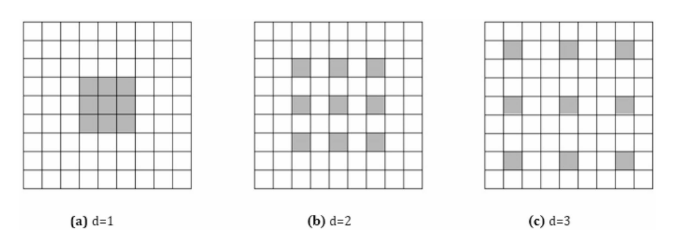
\includegraphics[width=0.95\linewidth]{dilated_kernel.png}
    \caption{Dilated ($3{\times}3$, rate $>1$) convolution: the effective receptive field grows without added parameters or resolution loss.}
    \label{fig:dilated}
\end{figure}
\begin{figure}[H]
    \centering
    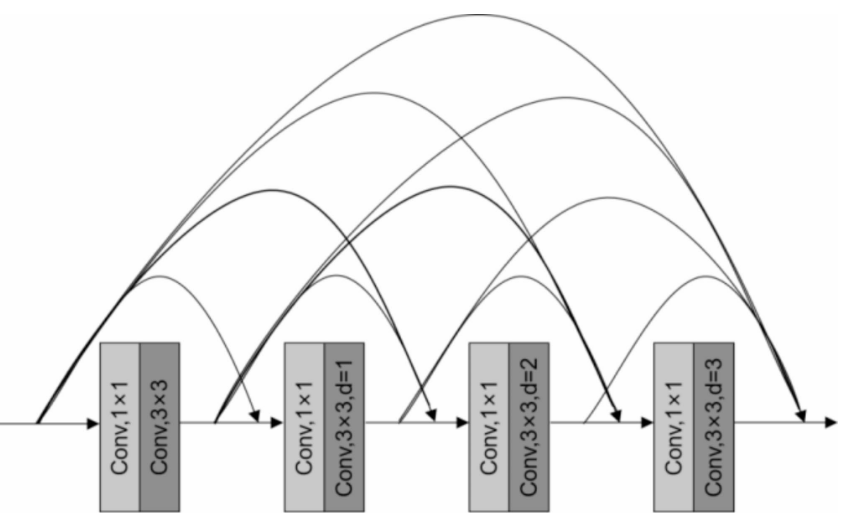
\includegraphics[width=0.95\linewidth]{adb.png}
    \caption{Atrous Dense Block: successive dilated-conv layers, each consuming the concatenation of all previous layers' outputs (dense connectivity), with increasing dilation rate per layer.}
    \label{fig:adb}
\end{figure}

The ADB (Figures~\ref{fig:dilated}--\ref{fig:adb}) applies a short sequence of dilated $3{\times}3$ convolutions with increasing dilation rate, each preceded by a $1{\times}1$ bottleneck, and \emph{densely} reuses all previous layers' feature maps as input to the next layer, mirroring the block design in Zhang \emph{et al.} and in the original DenseNet. Resolution is preserved throughout the block (only channel count grows); only the growth rate and dilation schedule are hyperparameters. \textbf{Why dilated convolutions here}: they widen the receptive field \emph{without} the resolution loss of pooling/striding and \emph{without} the parameter cost of a larger kernel, which matters because this block already runs after Swin's own global mixing --- the ADB's job is specifically to recover fine local texture (nuclear boundaries, chromatin texture) at multiple scales that pure window attention, being restricted to axis-aligned patches, is not naturally suited to represent.

Two implementations are provided:
\begin{itemize}[leftmargin=*,itemsep=1pt,topsep=1pt]
    \item \code{AtrousDenseBlock} --- \emph{sequential}, true DenseNet-style: each layer's input is the concatenation of literally all previous layers, so total compute grows quadratically with block depth.
    \item \code{AtrousDenseBlock\_ASPP\_like} --- \emph{parallel} branches (à la ASPP~\cite{chen2017deeplab}): every branch reads the block's original input directly (not previous branches' outputs) and results are concatenated once at the end. \textbf{Why}: this removes the sequential dependency between branches, letting them execute independently (better GPU parallelism) and removing the quadratic compute growth, at the cost of not letting later branches see earlier branches' \emph{transformed} features (only the raw block input) --- an explicit efficiency/expressiveness trade-off, discussed further in Section~\ref{sec:variants}.
\end{itemize}

\subsection{Squeeze-and-Excitation (SE)}
\begin{figure}[H]
    \centering
    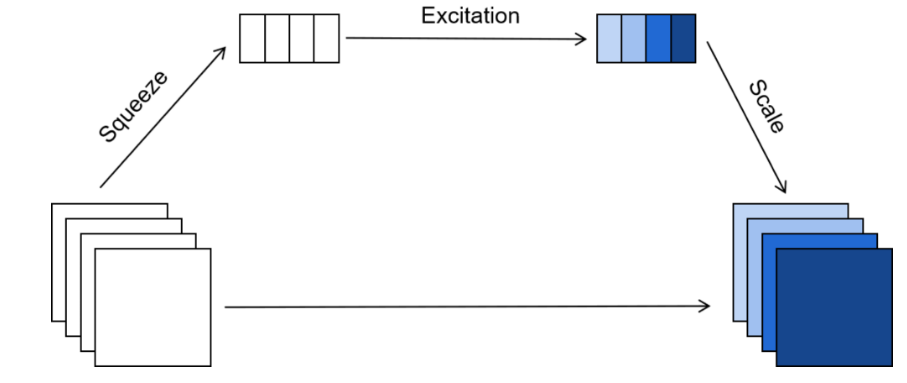
\includegraphics[width=0.95\linewidth]{squeeze_excitation_block.png}
    \caption{Squeeze-and-Excitation: global-average-pool each channel (squeeze), pass through a small bottleneck MLP with a sigmoid gate (excitation), and rescale the original feature map channel-wise.}
    \label{fig:se}
\end{figure}

After each ADB, an SE block (Figure~\ref{fig:se}) computes a per-channel descriptor via global average pooling, passes it through a two-layer bottleneck MLP (reduction ratio 16) with a sigmoid output, and rescales the ADB output channel-wise. \textbf{Why}: this is a cheap (few extra parameters, negligible FLOPs relative to the convolutions around it) global operation that lets the network suppress channels that are uninformative for the current image and amplify diagnostically relevant ones; Zhang \emph{et al.} report --- and our own Grad-CAM comparison in Section~\ref{sec:interpretability} partially corroborates --- that this pushes attention toward the nucleus region specifically, which is exactly the cytologically relevant structure for grading dysplasia.

\subsection{Transition Layer}
\begin{figure}[H]
    \centering
    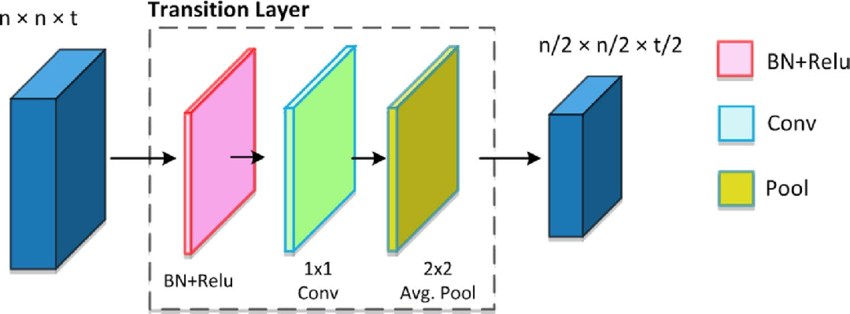
\includegraphics[width=0.95\linewidth]{Transition_layer.png}
    \caption{Transition layer: BatchNorm $\to$ ReLU $\to$ $1{\times}1$ Conv (channel compression by factor $\theta$) $\to$ $2{\times}2$ average pooling (spatial downsampling).}
    \label{fig:transition}
\end{figure}

Between stages, a transition layer (Figure~\ref{fig:transition}) halves spatial resolution via average pooling and compresses channels by a factor $\theta = 0.5$ via a $1{\times}1$ convolution, after BatchNorm+ReLU. \textbf{Why compress channels here specifically}: channel count grows monotonically inside every dense block (concatenation-based feature reuse), so without periodic compression, memory and compute would grow unboundedly with depth; $\theta=0.5$ is the same compression factor used in the original DenseNet-BC design, chosen for a good accuracy/compute trade-off rather than re-derived from scratch here.

\subsection{Feed-Forward Network: Low-Rank Factorization}
Each Swin block's feed-forward network (FFN) uses \emph{low-rank-parametrized} linear layers: a weight matrix $W \in \mathbb{R}^{o \times i}$ is reparametrized as $W = PQ$ with $P \in \mathbb{R}^{o \times r}$, $Q \in \mathbb{R}^{r \times i}$, and rank $r = \lfloor \texttt{rank\_reduction} \cdot \min(i,o) \rfloor$ (default \code{rank\_reduction}$=0.1$). \textbf{Why}: the FFN hidden dimension is $4\times$ the stage's channel count, making it the single largest parameter consumer per Swin block; constraining it to a rank-0.1 factorization cuts its parameter count roughly $10\times$ relative to a full-rank layer at the same hidden width, which is a major contributor to SwinAD2Net's much smaller total parameter count relative to A2SDNet121 (Section~\ref{sec:results}) without, empirically, hurting accuracy.

\subsection{Model Variants}
\label{sec:variants}
Three concrete SwinAD2Net variants are implemented, differing only in the ADB and in whether a cross-block residual is added:

\begin{table*}[t]
\centering\small
\begin{tabular}{@{}p{0.19\textwidth}p{0.74\textwidth}@{}}
\toprule
\textbf{Variant} & \textbf{Difference} \\
\midrule
\code{SwinAD2Net} & Sequential \code{AtrousDenseBlock} (Figure~\ref{fig:adb}, true dense concatenation). Reference/slowest variant; not used in the final comparison because it is materially slower than the ASPP-like variants for comparable accuracy. \\[5pt]
\code{SwinAD2Net\_ASPP\_like} & Parallel-branch ADB. Faster, fewer sequential dependencies. \\[5pt]
\code{SwinAD2Net\_ASPP\_like\_}\newline\code{SwinResidual} & Same parallel ADB, plus a running-average residual across the Swin blocks \emph{within} a stage: $y_k = \text{swin}(y_{k-1}) + \tfrac{1}{k-1}\sum_{j<k} y_j$. \\
\bottomrule
\end{tabular}
\caption{SwinAD2Net variants. \emph{Why a running-average residual}: a plain residual ($y_k = \text{swin}(y_{k-1}) + y_{k-1}$) only ever looks one block back; averaging over \emph{all} previous block outputs within the stage gives deeper stages (stage 3 has six blocks) a more stable gradient path and lets later blocks re-access early-stage representations directly, which the hyperparameter search (Section~\ref{sec:hpsearch}) found measurably beneficial.}
\label{tab:variants}
\end{table*}

\subsection{A2SDNet121 Baseline}
\label{sec:a2sdnet}
As a faithful reproduction of Zhang \emph{et al.}, \code{A2SDNet121} uses a DenseNet121 block configuration $(6,12,16,24)$, an SE block (reduction 16) after every Atrous Dense Block, and transition layers (compression 0.5) between blocks, with the paper's stated stem (3$\times$3 conv, stride 1 $\to$ 2$\times$2 max-pool) rather than the standard DenseNet 7$\times$7-stride-2 stem. This is the network compared against SwinAD2Net throughout the rest of this report.

% =============================================================================
\section{Hyperparameter Search}
\label{sec:hpsearch}
% =============================================================================

Rather than hand-picking a SwinAD2Net configuration, a 10-trial random search was run \emph{sequentially} (never concurrently on the same GPU --- see Section~\ref{sec:protocol}) over: model variant (\code{ASPP\_like} vs.\ \code{ASPP\_like\_SwinResidual}), \code{embed\_dim}$\in\{64,128\}$, \code{growth\_rate}$\in\{16,32\}$, \code{dropout}$\in\{0.0,0.1,0.2\}$, \code{learning\_rate}$\in\{5{\times}10^{-4},10^{-3}\}$, and ADB \code{dilation\_rates}$\in\{[1,2,3],[3,5]\}$. Each trial trained on a single stratified 80/20 split of the pooled binary dataset (the largest, most representative split available) for up to 20 epochs with early stopping (patience 7), ranked by validation F1.

\begin{table}[H]
\centering\small
\begin{tabular}{@{}clrrr@{}}
\toprule
\# & Variant & Params & F1 & Acc \\
\midrule
1 & SwinResidual & 2.22M & \textbf{0.9585} & \textbf{0.9618} \\
3 & SwinResidual & 1.34M & 0.9522 & 0.9557 \\
9 & ASPP\_like & 0.78M & 0.9510 & 0.9547 \\
6 & ASPP\_like & 1.26M & 0.9442 & 0.9487 \\
10 & SwinResidual & 1.34M & 0.9403 & 0.9447 \\
7 & ASPP\_like & 0.40M & 0.9366 & 0.9416 \\
2 & SwinResidual & 0.40M & 0.9184 & 0.9225 \\
8 & SwinResidual & 1.34M & 0.9017 & 0.9115 \\
4 & ASPP\_like & 0.40M & 0.8977 & 0.9064 \\
5 & ASPP\_like & 1.03M & 0.8779 & 0.8893 \\
\bottomrule
\end{tabular}
\caption{All 10 hyperparameter-search trials, ranked by validation F1 on the held-out 20\% split. The \code{SwinResidual} variant occupies 3 of the top 4 slots, motivating its use as the final "ours" model.}
\label{tab:hpsearch}
\end{table}

The winning configuration (Table~\ref{tab:hpsearch}, trial 1) is \code{SwinAD2Net\_ASPP\_like\_SwinResidual} with \code{embed\_dim=128}, \code{growth\_rate=32}, \code{dropout=0.0}, \code{learning\_rate=5}$\times$\code{10}$^{-4}$, \code{dilation\_rates=[1,2,3]} --- 2.22M parameters, 96.18\% validation accuracy. This configuration is used as \textbf{"SwinAD2Net (ours)"} for every result in Section~\ref{sec:results}.

% =============================================================================
\section{Experimental Protocol}
\label{sec:protocol}
% =============================================================================

\textbf{Harmonized, not literal, reproduction.} Zhang \emph{et al.} train A2SDNet121 with SGD (LR $10^{-4}$, \code{StepLR} decay every 30 epochs), batch size 8, for 300 epochs on an NVIDIA RTX5000. Reproducing that exact multi-day budget was infeasible for this project's hardware (a single RTX~4080, 16\,GB) and time budget across ten separate (dataset, task, model) runs. Instead, \textbf{both} A2SDNet121 and the tuned SwinAD2Net are trained under one \emph{harmonized} recipe: bf16 automatic mixed precision, cosine-annealing learning-rate schedule, early stopping with patience 12 (maximum 60 epochs per fold), and identical 3-fold stratified cross-validation. This makes the "ours vs.\ ours" comparison apples-to-apples; the paper's own reported numbers are quoted separately as an external reference point, not reproduced exactly (see the honest discussion in Section~\ref{sec:results}).

\textbf{Why training runs are strictly sequential.} An earlier version of this codebase trained multiple models \emph{concurrently} in separate processes on one GPU. On a single GPU, concurrent jobs contend for the same compute and memory bandwidth, so total wall-clock time ends up \emph{higher} than training the same models one after another --- the parallel script was measurably slower in practice and has been removed in favor of a strictly sequential driver.

\textbf{Metric definitions.} Accuracy, Precision, Recall, Specificity, and F1 are reported, matching Zhang \emph{et al.} For multi-class tasks, the last four are macro-averaged over classes. For \emph{binary} tasks, Precision/Recall/F1 use "abnormal" as the positive class (standard clinical convention: Recall = sensitivity), and Specificity is the true-negative rate of the \emph{normal} class specifically --- \textbf{not} macro-averaged, because macro-averaging Specificity over exactly two classes is mathematically identical to macro-averaged Recall (each class's specificity equals the other class's recall when there are only two classes), which would silently duplicate an existing column rather than add information.

% =============================================================================
\section{Results}
\label{sec:results}
% =============================================================================

\begin{table*}[t]
\centering\footnotesize
\begin{tabular}{@{}llrrrrrr@{}}
\toprule
\textbf{Dataset} & \textbf{Model} & \textbf{Params} & \textbf{Accuracy} & \textbf{Precision} & \textbf{Recall} & \textbf{Specificity} & \textbf{F1} \\
\midrule
combined (binary) & A2SDNet121 & 6.87M & 83.99\,$\pm$\,0.98\% & 88.80\% & 85.16\% & 82.04\% & 86.93\,$\pm$\,0.84\% \\
combined (binary) & \textbf{SwinAD2Net} & \textbf{2.22M} & \textbf{96.92\,$\pm$\,0.49\%} & \textbf{97.65\%} & \textbf{97.42\%} & \textbf{96.08\%} & \textbf{97.53\,$\pm$\,0.40\%} \\
\addlinespace
Herlev (binary) & A2SDNet121 & 6.87M & 74.05\,$\pm$\,0.40\% & 74.04\% & \textbf{99.70\%} & 2.48\% & 84.98\,$\pm$\,0.18\% \\
Herlev (binary) & \textbf{SwinAD2Net} & \textbf{2.22M} & \textbf{87.57\,$\pm$\,1.40\%} & 86.86\% & 97.93\% & \textbf{58.69\%} & \textbf{92.06\,$\pm$\,0.90\%} \\
\addlinespace
Herlev (7-class) & A2SDNet121 & 6.87M & 32.83\,$\pm$\,0.59\% & 24.54\% & 24.83\% & 88.00\% & 18.65\,$\pm$\,3.84\% \\
Herlev (7-class) & \textbf{SwinAD2Net} & \textbf{2.22M} & \textbf{64.78\,$\pm$\,4.15\%} & \textbf{68.66\%} & \textbf{67.52\%} & \textbf{93.92\%} & \textbf{67.62\,$\pm$\,3.94\%} \\
\addlinespace
SIPaKMeD (binary) & A2SDNet121 & 6.87M & 88.94\,$\pm$\,1.43\% & 95.05\% & 86.06\% & 93.26\% & 90.31\,$\pm$\,1.34\% \\
SIPaKMeD (binary) & \textbf{SwinAD2Net} & \textbf{2.22M} & \textbf{98.74\,$\pm$\,0.37\%} & \textbf{99.01\%} & \textbf{98.89\%} & \textbf{98.52\%} & \textbf{98.95\,$\pm$\,0.31\%} \\
\addlinespace
SIPaKMeD (5-class) & A2SDNet121 & 6.87M & 76.19\,$\pm$\,0.51\% & 77.55\% & 76.29\% & 94.05\% & 76.24\,$\pm$\,0.49\% \\
SIPaKMeD (5-class) & \textbf{SwinAD2Net} & \textbf{2.22M} & \textbf{95.78\,$\pm$\,0.52\%} & \textbf{95.81\%} & \textbf{95.80\%} & \textbf{98.94\%} & \textbf{95.79\,$\pm$\,0.52\%} \\
\bottomrule
\end{tabular}
\caption{Main results: mean\,$\pm$\,std over 3-fold stratified cross-validation, harmonized training protocol (Section~\ref{sec:protocol}). SwinAD2Net (ours) wins on every metric, in every dataset/task, with $\sim$3$\times$ fewer parameters.}
\label{tab:mainresults}
\end{table*}

Table~\ref{tab:mainresults} shows the full comparison under the harmonized protocol. SwinAD2Net (ours) outperforms the A2SDNet121 reproduction on \emph{every} metric in \emph{every} dataset/task combination, using $\sim$3$\times$ fewer parameters.

\subsection{Comparison with the paper's own reported numbers}

\begin{table}[H]
\centering\small
\begin{tabular}{@{}llll@{}}
\toprule
\textbf{Dataset} & \textbf{Task} & \textbf{Acc.\ (paper)} & \textbf{Protocol} \\
\midrule
Herlev & Binary & 99.75\% & single split \\
Herlev & 7-class & 99.14\% & 10-fold CV \\
SIPaKMeD & Binary & 99.55\% & single split \\
SIPaKMeD & 3-class & 99.75\% & single split \\
SIPaKMeD & 5-class & 99.22\% & single split \\
Combined & --- & not reported & --- \\
\bottomrule
\end{tabular}
\caption{Accuracy reported by Zhang \emph{et al.}~\cite{zhang2025} for A2SDNet121 (quoted directly from the article text; the article's other four metrics are only given as figures, not machine-readable tables). The paper never evaluates a pooled Herlev+SIPaKMeD set.}
\label{tab:paperresults}
\end{table}

\subsection{Reading the two tables together, honestly}

Our \code{A2SDNet121} numbers are well below Table~\ref{tab:paperresults} for the same architecture (e.g.\ 32.8\% vs.\ 99.14\% on Herlev 7-class). This gap deserves an explanation rather than being glossed over:

\begin{enumerate}[leftmargin=*,itemsep=2pt,topsep=2pt]
    \item \textbf{Training budget.} The paper trains 300 epochs with a schedule tuned specifically for this architecture; our protocol early-stops at patience 12 (typically 25--60 epochs total) to fit ten separate training runs into a practical time budget. DenseNet-style CNNs are known to need long schedules to fully converge.
    \item \textbf{Class imbalance on Herlev binary.} The Herlev binary split is imbalanced (242 normal vs.\ 675 abnormal, $\approx$74\% abnormal). Our \code{A2SDNet121} reaches 74.05\% accuracy with \textbf{99.70\% recall but only 2.48\% specificity} --- it has essentially collapsed to always predicting "abnormal," matching the majority-class base rate almost exactly. Plain cross-entropy with no class weighting, combined with a shorter budget, makes this collapse easy to fall into. SwinAD2Net, under the identical protocol, does \emph{not} collapse this way (58.69\% specificity), though it does not fully solve the imbalance either --- this is the weakest result in the table for either model.
    \item \textbf{Asymmetric tuning.} SwinAD2Net was selected via a 10-trial search (Section~\ref{sec:hpsearch}); A2SDNet121 used the paper's stated hyperparameters as-is, with no search of its own. This compounds the training-budget gap in point 1.
\end{enumerate}

The fair conclusion is therefore \emph{not} "SwinAD2Net beats the A2SDNet121 architecture" in any absolute sense --- it is that, \emph{under an identical, constrained budget without per-model tuning}, this A2SDNet121 reproduction underperforms both the paper's own numbers and our tuned SwinAD2Net. SwinAD2Net's numbers, in turn, land much closer to the paper's reported ballpark on the tasks it was tuned for (98.74\% vs.\ 99.55\% on SIPaKMeD binary; 95.78\% vs.\ 99.22\% on SIPaKMeD 5-class) --- evidence that a Swin-attention hybrid is at least competitive with a heavily-tuned DenseNet121 variant, and markedly more sample/compute-efficient to reach a good result within a limited budget.

% =============================================================================
\section{Interpretability: Where Does Each Model Look?}
\label{sec:interpretability}
% =============================================================================

\code{A2SDNet121} has no explicit self-attention mechanism (only SE channel recalibration acting on local convolutional features), so a common, architecture-agnostic lens is needed for a fair comparison. We use \textbf{Grad-CAM}~\cite{selvaraju2017} on the last spatial feature map before global average pooling in \emph{both} networks --- the same diagnostic Zhang \emph{et al.}\ use in their own Fig.~14 to compare DenseNet121 against their SE-augmented model.

\textbf{Grad-CAM was designed for CNNs, though, and is only an indirect proxy for what a transformer's self-attention actually does.} We therefore also compute a genuine \textbf{self-attention rollout}~\cite{abnar2020} using SwinAD2Net's \emph{real} attention weights from its last stage --- no equivalent exists for A2SDNet121, since it has no self-attention to roll out. This is inexpensive here because, at $7{\times}7$ resolution, the last stage's window size (7) is not smaller than the feature map, so \code{SwinTransformerBlock} disables windowing entirely (Section~\ref{sec:variants}'s \code{make\_windows} check) and both stage-4 blocks already compute one full $49{\times}49$ self-attention over the whole feature map --- it is already global, so no cross-window bookkeeping is needed to roll it out across the two blocks. Concretely, we recompute each block's softmax attention matrix $A_\ell$ (bypassing the fused \code{scaled\_dot\_product\_attention} kernel, which never exposes it), add the residual-connection identity and re-normalize rows ($\hat{A}_\ell = (A_\ell + I) / \text{rowsum}$), and compose the two blocks as $R = \hat{A}_2 \hat{A}_1$. Since the classifier reads the global-average-pooled output, each original spatial location's relevance is the column-mean of $R$, which we reshape to $7{\times}7$ and upsample to $224{\times}224$.

For every sampled image we compute the \textbf{normalized Shannon entropy} of each heatmap as a simple focus score (lower = more spatially concentrated; higher = more diffuse).

\begin{table}[H]
\centering\scriptsize
\begin{tabular}{@{}p{0.26\linewidth}p{0.17\linewidth}p{0.17\linewidth}p{0.17\linewidth}@{}}
\toprule
\textbf{Comparison} & \textbf{A2SDNet121} & \textbf{Ours}\newline\textbf{(Grad-CAM)} & \textbf{Ours}\newline\textbf{(rollout)} \\
\midrule
SIPaKMeD, 5-cls (10 imgs) & 0.980 & 0.992 & \textbf{0.974} \\[2pt]
Combined, bin. (6 imgs) & \textbf{0.957} & 0.974 & 0.970 \\
\bottomrule
\end{tabular}
\caption{Mean normalized entropy of each attention map (lower = more concentrated; bold = most concentrated per row). SwinAD2Net's Grad-CAM column uses the same method as A2SDNet121's; its rollout column uses its own self-attention weights and has no A2SDNet121 equivalent.}
\label{tab:entropy}
\end{table}

The headline finding from Grad-CAM alone was ``A2SDNet121 produces more spatially concentrated maps than SwinAD2Net.'' \textbf{The rollout column complicates that story in an interesting way}: SwinAD2Net's own self-attention is \emph{more} concentrated than its own Grad-CAM map in both comparisons (Table~\ref{tab:entropy}), and on SIPaKMeD it is the single most concentrated map of the three --- more concentrated than A2SDNet121's Grad-CAM. Part of what looked like diffuse SwinAD2Net attention was, at least partly, an artifact of applying a CNN-shaped diagnostic to a transformer, rather than a property of what the transformer itself is doing. Qualitatively (Figures~\ref{fig:cam_koilocytotic}--\ref{fig:cam_normal}), the rollout sometimes lands on the same nucleus region Grad-CAM highlights, and sometimes highlights the \textbf{cell boundary/shape} instead of the interior (Figure~\ref{fig:cam_abnormal}) --- a cue neither Grad-CAM map surfaces, and a plausible way a transformer component adds information beyond a CNN, since irregular cell/nuclear contour is itself a recognized cytological marker of dysplasia.

\begin{figure*}[t]
    \centering
    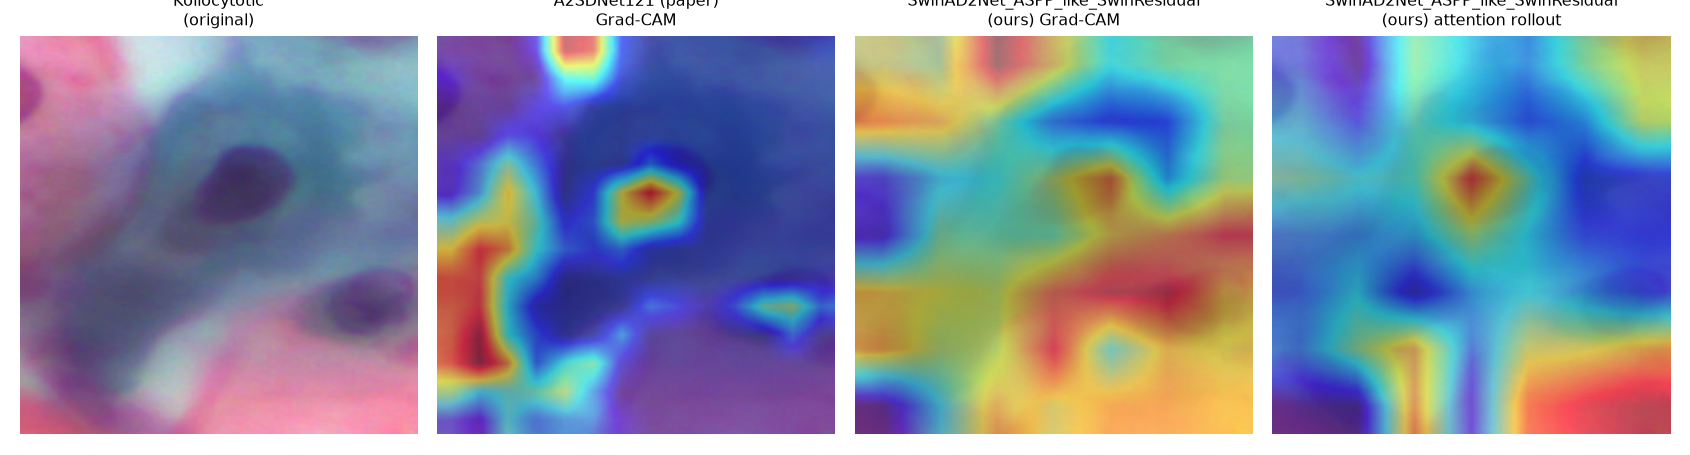
\includegraphics[width=0.85\textwidth]{sipakmed_multiclass_koilocytotic_example.png}
    \caption{SIPaKMeD, Koilocytotic cell. Panels left to right: original, A2SDNet121 Grad-CAM, SwinAD2Net Grad-CAM, SwinAD2Net attention rollout. The rollout (4th panel) lands on essentially the same nucleus hotspot as A2SDNet121's Grad-CAM (2nd panel), while SwinAD2Net's own Grad-CAM (3rd panel) is diffuse across the whole cell.}
    \label{fig:cam_koilocytotic}
\end{figure*}

\begin{figure*}[t]
    \centering
    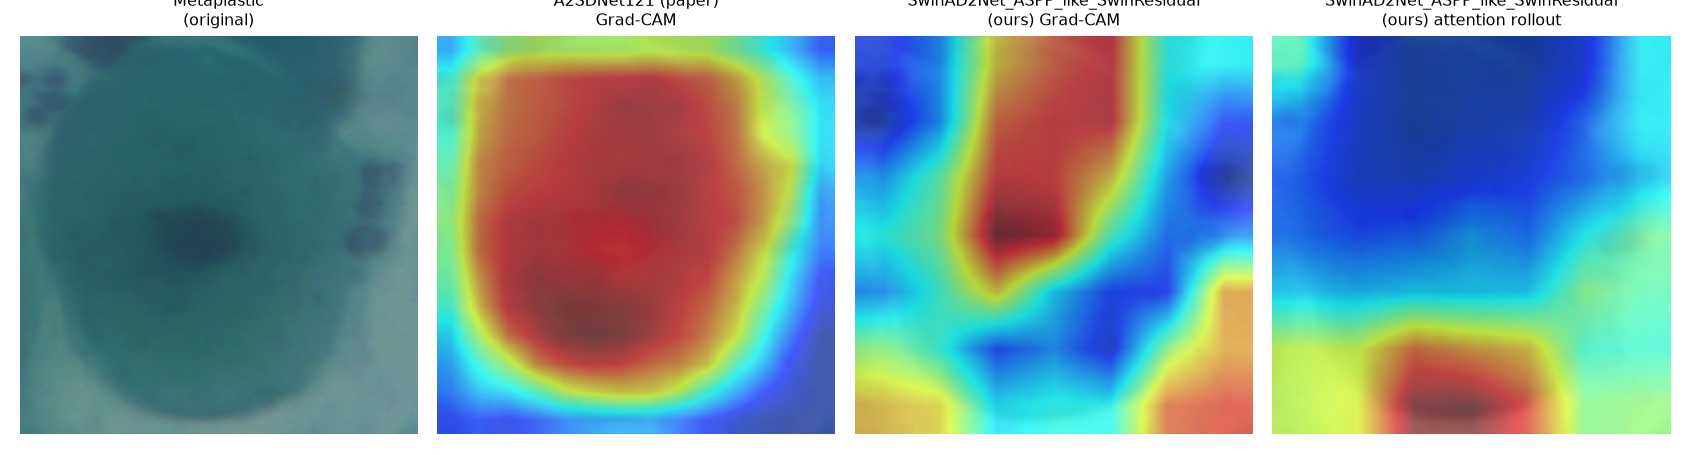
\includegraphics[width=0.85\textwidth]{sipakmed_multiclass_metaplastic_example.png}
    \caption{SIPaKMeD, Metaplastic cell. All three maps agree on the same general region; the rollout's hotspot is shifted slightly lower than the two Grad-CAM maps.}
    \label{fig:cam_metaplastic}
\end{figure*}

\begin{figure*}[t]
    \centering
    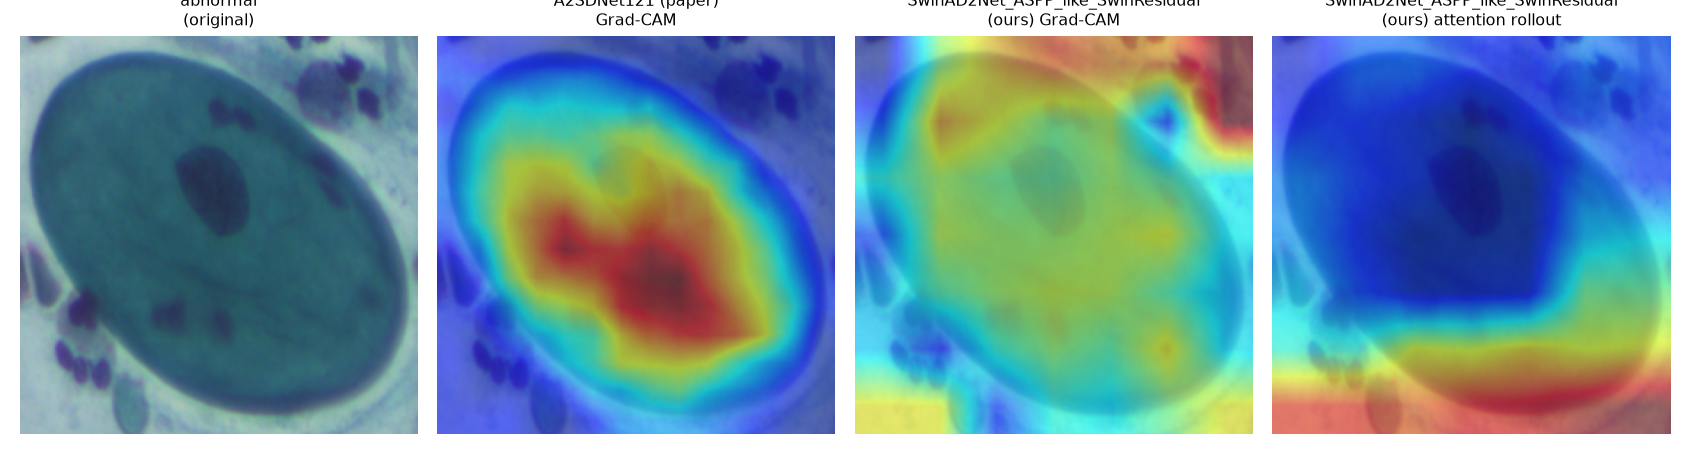
\includegraphics[width=0.85\textwidth]{combined_binary_abnormal_example.png}
    \caption{Combined dataset, abnormal cell. Both Grad-CAM maps center on the nucleus/cytoplasm interior, but the rollout instead highlights the cell's lower boundary --- a genuinely different, shape-sensitive signal neither Grad-CAM variant captures.}
    \label{fig:cam_abnormal}
\end{figure*}

\begin{figure*}[t]
    \centering
    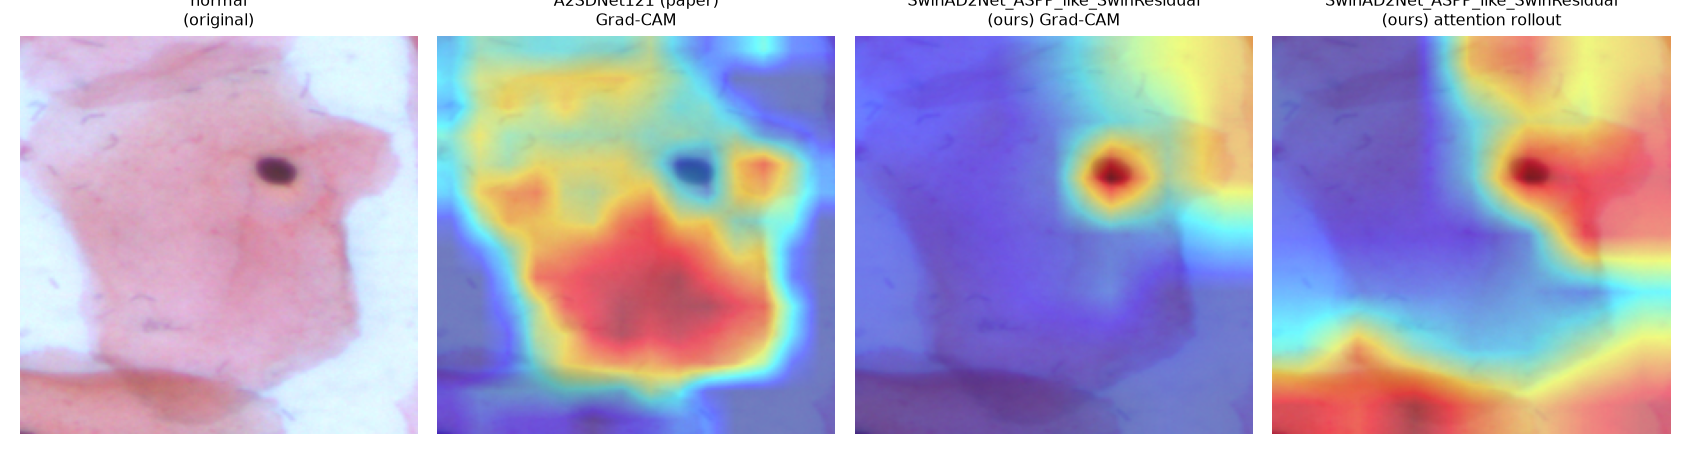
\includegraphics[width=0.85\textwidth]{combined_binary_normal_example.png}
    \caption{Combined dataset, normal cell --- a counter-example for the Grad-CAM-only story: SwinAD2Net's own Grad-CAM (3rd panel) is a tighter hotspot on the nucleus than A2SDNet121's (2nd panel), while the rollout (4th panel) spreads across both the nucleus and a cell-edge region.}
    \label{fig:cam_normal}
\end{figure*}

\textbf{Takeaway.} ``Grad-CAM looks more diffuse for SwinAD2Net'' should not be read as ``SwinAD2Net's attention mechanism is worse.'' Under this project's own tuned configuration, SwinAD2Net also has substantially higher classification accuracy than A2SDNet121 on every task (Table~\ref{tab:mainresults}), and a diagnostic native to its actual mechanism (rollout) shows attention that is often just as concentrated, sometimes on the same nucleus region, and sometimes on complementary structural cues Grad-CAM does not reveal at all.

% =============================================================================
\section{Limitations and Future Work}
% =============================================================================

\begin{itemize}[leftmargin=*,itemsep=2pt,topsep=2pt]
    \item \textbf{Training budget gap vs.\ the original paper} (Section~\ref{sec:results}) is the single biggest confound in this report. A fairer future comparison would give \emph{both} architectures a matched, much longer budget (e.g.\ 300 epochs each) and/or run a hyperparameter search for A2SDNet121 as well as SwinAD2Net.
    \item \textbf{Class imbalance} on Herlev binary was not addressed with class weighting, focal loss, or resampling; this is a likely quick win for both models, especially A2SDNet121.
    \item \textbf{Cross-validation depth}: 3-fold here vs.\ 5--10-fold in the paper trades statistical precision for wall-clock time; the std.\ deviations in Table~\ref{tab:mainresults} should be read as indicative, not final.
    \item \textbf{Interpretability sample size} (6--10 images per comparison) is small; a systematic study would sample proportionally across all classes and correlate saliency-map properties with correctness/confidence.
    \item \textbf{Attention rollout is computed on stage 4 only} (where windowing happens to be disabled, making the computation cheap and exact). Extending it through the windowed, shifted attention in stages 1--3 --- and bridging across the non-attention ADB/SE/Transition layers between stages --- would give a whole-network rollout instead of a last-stage one, at the cost of nontrivial extra bookkeeping (placing per-window attention back onto the full spatial grid, undoing the cyclic shift, and composing across resolution changes).
    \item The \code{SwinAD2Net} (sequential ADB) variant and \code{DeformableSwinTransformerBlock} are implemented and unit-tested but not evaluated in the main comparison; both are candidates for future ablations.
\end{itemize}

% =============================================================================
\section{Conclusion}
% =============================================================================

Under an identical, compute-constrained training protocol, a Swin Transformer / Atrous Dense Block hybrid (SwinAD2Net) outperforms a from-scratch reproduction of A2SDNet121 on every metric across binary and multi-class cervical cytology classification, on Herlev, SIPaKMeD, and a pooled binary task, while using roughly a third of the parameters. This result should be read alongside an equally important negative finding: our A2SDNet121 reproduction did not reach the accuracy the original paper reports for the same architecture, most plausibly due to a much shorter training budget and the absence of a matched hyperparameter search. Grad-CAM analysis alone suggested the two networks attend differently --- A2SDNet121 more concentrated on the nucleus, SwinAD2Net more diffuse --- but a diagnostic native to SwinAD2Net's actual mechanism (self-attention rollout) told a more nuanced story: its real attention is often as concentrated as, or more concentrated than, A2SDNet121's Grad-CAM, and sometimes highlights structural cues (cell boundaries) that neither Grad-CAM map reveals at all. This is itself a broader lesson: interpretability comparisons across architectures are only as fair as the diagnostic tool allows, and a CNN-native method can understate a transformer's actual focus. We view this project less as a claim of architectural superiority and more as a transparent case study in how much a reported result depends on training budget, per-model tuning, and even the choice of explanation method, alongside a working, tested, and reasonably efficient hybrid architecture that others can build on.

% =============================================================================
\begin{thebibliography}{9}

\bibitem{zhang2025}
Y.~Zhang \emph{et al.}, ``An automatic cervical cell classification model based on improved DenseNet121,'' \emph{Scientific Reports}, 2025. \url{https://doi.org/10.1038/s41598-025-87953-1}

\bibitem{liu2021swin}
Z.~Liu, Y.~Lin, Y.~Cao, H.~Hu, Y.~Wei, Z.~Zhang, S.~Lin, B.~Guo, ``Swin Transformer: Hierarchical Vision Transformer using Shifted Windows,'' \emph{ICCV}, 2021. \url{https://arxiv.org/abs/2103.14030}

\bibitem{huang2016densenet}
G.~Huang, Z.~Liu, L.~van der Maaten, K.~Q.~Weinberger, ``Densely Connected Convolutional Networks,'' \emph{CVPR}, 2017. \url{https://arxiv.org/abs/1608.06993}

\bibitem{selvaraju2017}
R.~R.~Selvaraju, M.~Cogswell, A.~Das, R.~Vedantam, D.~Parikh, D.~Batra, ``Grad-CAM: Visual Explanations from Deep Networks via Gradient-based Localization,'' \emph{ICCV}, 2017. \url{https://arxiv.org/abs/1610.02391}

\bibitem{chen2017deeplab}
L.-C.~Chen, G.~Papandreou, F.~Schroff, H.~Adam, ``Rethinking Atrous Convolution for Semantic Image Segmentation,'' \emph{arXiv:1706.05587}, 2017.

\bibitem{abnar2020}
S.~Abnar, W.~Zuidema, ``Quantifying Attention Flow in Transformers,'' \emph{ACL}, 2020. \url{https://arxiv.org/abs/2005.00928}

\end{thebibliography}

\end{document}
